\chapter{Метод Кунченка}

Відомо, що поліном Тейлора є одним з найкращих способів апроксимації функції на деякому інтервалі, проте задля
використання цього методу необхідно забезпечити $n$-раз гладкість функції.

Кунченком~Ю.\,П. було запропоновано використовувати для апроксимації поліном, побудований з неортонормованого базису
функцій, що були отримані шляхом певних перетворень з шаблона.

В цьому розділі буде запропонований метод пошуку шаблонів за допомогою апроксимації поліномів у просторі Кунченко.
Для цього буде розглянутий лінійній простір Кунченко, метод розкладання довільної функції в цьому просторі й
застосування цього розкладення в проблемі пошуку шаблонів.
Також будуть розглянуті методи, за допомогою яких можна поліпшити результати алгоритму.

\section{Лінійній простір Кунченка}
    Нехай $f(x)$ --- так звана породжуюча функція, що визначена на проміжку ${[a, d]}$, а $\{ \phi_v( x ) \}$ ---
    довільна множина функціональний перетворень.
    Тоді, можна породити множину функцій
    \begin{equation}
        u_v(x) = \phi_v( f( x ))
    \end{equation}

    З цієї множини можна вибрати підмножину лінійно"=незалежних функцій.
    Лінійний простір, утворений на такій множині, називатимемо лінійним простором над незалежними породженими
    функціями, або лінійний простором Кунченка (LFKu).

    На цьому просторі можна звичайним чином визначити скалярний добуток:
    \begin{equation}
        \Psi_{v,k} = (u_v( x ), u_k( x ) ) = \int\limits_a^d u_v( x ) u_k( x )\,\mathrm{d}x,
    \end{equation}
    та відстань між двома елементами:
    \begin{equation}
        \rho_{v,k}^2 = \|u_v( x ) - u_k( x )\|^2 = \int\limits_a^d\left(u_v(x) - u_k(x)\right)^2\,\mathrm{d}x
    \end{equation}

    Виберемо деяку породжену функцію $u_b(x)$, яку будемо називати основною.
    Тоді множину функцій $u_v(x), v \ne b$ будемо називати доповнювальними функціями.

    Можна утворити поліном Кунченка з доповнювальних функцій:
    \begin{equation}
        \label{eq:polynom}
        P_t( x ) = \sum^t_{k = 1, k \ne b} a_k u_k( x  )
    \end{equation}

    Відстань між основною функцією $u_b(x)$ та утвореним поліномом за визначенням буде дорівнювати:
    \begin{equation}
        \rho^2_{b,P} = \int\limits_a^d\left( u_b(x) - P_t(x)\right)^2 \, \mathrm{d}x
    \end{equation}

    Можна показати, що коефіцієнти $a_k, k \ne 0$ знаходяться з системи лінійних рівнянь:
    \begin{equation}
        \label{eq:linear-system}
        \sum^t_{k=1,k\ne b} a_k F_{v,k} = F_{v,b},\qquad v=\overline{0,t}, v \ne b,
    \end{equation}
    де
    \begin{align}
        \label{eq:centered-correlants}
        F_{v,k} &\equiv \Psi_{v,k} - \Psi_v \Psi_k \| u_0( x ) \|^2\\
        \Psi_v &\equiv \frac{\Psi_{v,0}}{\left\|u_0(x)\right\|^2}\\
        a_0 &= \Psi_b - \sum\limits_{v=1, v \ne b}^r{a_v \Psi_v}
    \end{align}

    Спростив вираз, отримаємо:
    \begin{equation}
        \rho^2_{bP} = F_{b,b} - J_t,
    \end{equation}
    де $J_t$ --- інфоркуна полінома, що має вигляд:
    \begin{equation}
        J_t \equiv \sum_{v=1,v\ne b}^t a_v F_{v,b}
    \end{equation}

    Тоді мірою апроксимації поліномом будемо вважати наступну величину:
    \begin{equation}
        \label{eq:et}
        e_t = \frac{J_t}{\int\limits_a^d (u_b(x)-\Psi_b u_0( x ))^2\, \mathrm{d}x}
    \end{equation}

\section{Застосування розкладення для пошуку шаблону в сигналі}
    Візьмемо в якості породжуючої функції шаблон $f(x)$, що є визначеним на проміжку $\forall x_i \in {[a, d]}$.
    Тоді, нехай $\{u_v(x)\}$, також визначені $\forall x_i \in {[a, d]}$ --- породжені функції від шаблону, що
    утворюють лінійній простір Кунченко.

    Якщо взяти за основну функцію $u_b(x)$ вхідний сигнал на проміжку ${[a,d]}$, за допомогою~\eqref{eq:polynom} можна
    побудувати поліном наближення сигналу $P_t(x)$.

    Оскільки поліном, визначений таким чином буде являти собою наближення вхідного сигналу за допомогою певних
    перетворень з шаблону, то можна вважати величину~\eqref{eq:et} мірою схожості вхідного сигналу до шаблону на
    обраному проміжку.

    Таким чином, скомбінував метод ковзаючого вікна (розділ~\ref{ss:sliding-window}) з розкладенням сигналу в
    лінійному просторі Кунченко, можна отримати ефектограму, тобто функцію $e_t(x)$, що буде характеризувати схожість
    вхідного сигналу зі шаблоном у певному вікні.

    Оскільки ефектограма може приймати значення від $-1$ до $1$, можливо визначити поріг $e_0$, такий, що значення
    більше (або менше при умові його від’ємності) буде характеризувати відповідне вікно як таке, що містить
    модифікований шаблон.

    Цей алгоритм потребує наступні обчислення:
    \begin{itemize}
        \item $O(t^2) O(k^2)$ обчислень для підрахунку попарних центрованих корелянт~\eqref{eq:centered-correlants}
            всіх породжених функцій (кожна з яких має $k$ значень).
            Ця дія має бути виконаною лише один раз на початку пошуку, оскільки при ковзанні вікна вони не будуть
            змінюватись.
        \item $O(t) O(k)$ обчислень для підрахунку корелянт із основною функцією (вхідним сигналом)~$F_{v,b}$ на
            кожному кроці, оскільки значення основної функції змінюється із зсувом вікна.
        \item $O(t^3)$ обчислень для пошуку коренів системи лінійних рівнянь~\eqref{eq:linear-system}.
        \item $O(t) + O(k^2)$ для обрахування ефективності наближення на кожному кроці.
    \end{itemize}

\section{Методи покращення пошуку шаблонів}
    Як видно з попередніх обчислень, запропонований метод має більшу обчислювальну складність, ніж метод із
    використанням нормалізованої взаємокореляції (розділ~\ref{s:existing-compare}).

    В цьому підрозділі будуть запропоновані методи прискорення роботи алгоритму.

    \subsection{Пірамідальний пошук}
        Оскільки основною складовою кількості обчислень можна вважати $O(k^2)$, було запропоновано використання методу
        так званого пірамідального пошуку.
        \todo[inline]{Vanderbrug, G.J. and Rosenfeld, A. (1977) Two-stage Template Matching. IEEE Transactions on Computers, C-26,}
        \todo[inline]{Rosenfeld, A. and Vanderbrug, G.J. (1977) Coarse-Fine Template Matching. IEEE Transactions on Systems, Man and Cybernetics, 7, 104-107.}

        Ідея цього методу полягає в тому, що спочатку виконується певне масштабування (стиснення) шаблону та сигналу.
        Після цього виконується пошук стисненого шаблону в стисненому сигналі.
        Якщо знаходяться екстремуми, що характеризують знахідку шаблону, то на відповідній області нестисненого
        сигналу виконується пошук нестисненого шаблону.

        Таким чином, якщо сигнал та шаблон були промасштабовані із співвідношенням $1:10$, то головна складова
        кількості обчислень зміниться до $\frac{1}{100} O(k^2)$.
        Як правило, після першого етапу залишається значно менше областей, в яких потрібно уточнювати результат.

        Також варто зазначити, що можливі два підходи щодо стиснення сигналів:
        \begin{itemize}
            \item Зміна частоти дискретизації (resampling).
                В цьому випадку можна використовувати, наприклад фільтр Ланцоша, якщо орігінальна частота
                дискретизації не ділиться на нову.
                Проте значно ефективніше обирати таку нову частоту дискретизації, що ділить орігінальну частоту
                націло.
                В такому випадку можна вибрати кожне $m$-те значення сигналу та шаблону, де $m$ --- співвідношення
                частот.
                \todo[inline]{Ken Turkowski and Steve Gabriel (1990). "Filters for Common Resampling Tasks". In Andrew
                    S. Glassner. Graphics Gems I. Academic Press. pp. 147–165. ISBN 978-0-12-286165-9.}
            \item Брати середнє значення від деякого околу точки.
        \end{itemize}
    \subsection{Метод прискореного ковзання}
        Оскільки в процесі пошуку шаблону отримуємо функціональну залежність $e_t(x)$, що характеризує ступінь
        наближення вхідного сигналу певними модифікаціями шаблону, можна розглядати задачу цього пошуку як задачу
        оптимізації.

        Найбільш ефективним застосуванням методів оптимізації буде використання алгоритм пошуку інтервалів, що могуть
        містити екстремум функції ефективності наближення.
        Такий алгоритм можна зображено на малюнку~\ref{fig:svenn-algorithm}.

        \stepcounter{figurecount}
        \begin{figure}[!h]
            \centering
            
\includegraphics[height=0.85\textheight]{svenn.eps}
            \caption{Блок"=схема роботи алгоритму пошуку інтервалу з екстремумом}
            \label{fig:svenn-algorithm}
        \end{figure}

        Використовуючи цей алгоритм можна знайти інтервал, що містить певний екстремум, а потів уточнювати отримане
        значення.
        Цього можна досягти як повним обчисленням всіх значень функції $e_t(x)$ на отриманому проміжку, так і
        використанням методів уточнення інтервалів, таких як методи дихотомії та золотого перетину.

        Методи дихотомії та золотого перетину дозволяють уточнити (звузити) інтервал, що містить екстремум.
        Алгоритм методу золотого перетину має наступний вид:
        \begin{enumerate}
            \item Задати
                \begin{align*}
                    x_0 &= a\\
                    x_1 &= b\\
                \end{align*}
            \item Обчислити
                \begin{align*}
                    x_l &= x_1 - \frac{x_1 - x_0}{\phi}\\
                    x_r &= x_0 + \frac{x_1 - x_0}{\phi},
                \end{align*}
                де $\phi = \frac{1 + \sqrt{ 5 }}{2}$ --- пропорція золотого перетину.
            \item\label{enum:step3} Якщо $f(x_l) < f(x_r)$, то задати $x_0 = x_l$, інакше $x_1 = x_r$.
            \item Перевірити умови зупинки (наприклад, $\|x_1 - x_0\| < \varepsilon$).
                Якщо умова не виконується, то перейти до кроку~\ref{enum:step3}, інакше повернути інтервал ${[x_0,
                    x_1]}$ або $\frac{x_0+x_1}{2}$ в залежності від потреб задачі.
        \end{enumerate}

        Слід зазначити, що в залежності від природи сигналу та шаблону, функція ефективності наближення може мати
        різкі спади, а тому є сенс обмежити максимально можливий крок, який можна пропустити при пошуку інтервалу, що
        може містити шаблон.
\section{Пошук шаблонів в мовленнєвих сигналах}
    Обраний метод пошуку шаблонів має меншу чутливість до зміни шаблону, ніж інші методи.
    Розглянемо застосування цього методу до задачі пошуку шаблону в мовленнєвому сигналі, оскільки шаблони в сигналах
    такого типу (деяка мовленнєва одиниця) зазвичай
    \todo[inline]{Закінчити речення}

    Мовлення отримується за рахунок зміни в часі голосового тракту.
    Через це мовленнєвий сигнал має нестаціонарну природу.
    Оскільки при обробці сигналів найчастіше вважається, що амплітуда коливань є більш-менш незалежною від часу, то
    використання цих методів стає неприпустимим при обробці мовленнєвих сигналів.
    Використання таких методів до мовленнєвих сигналів буде мати дуже мало практичного значення.
    Наприклад, обчислення енергії сигналу є фундаментальним інструментом при обробці сигналів:
    \begin{equation}
        E_T = \sum\limits_{n = {-\infty}}^\infty{s^2\left(n\right)}
    \end{equation}

    Енергія сигналу є корисним інструментом у випадку, колу сигнал має обмежену енергію.
    Обчислення енергії мовленнєвого сигналу буде мати дуже малу практичну цінність, адже мовленнєвий сигнал за
    природою має енергію та амплітуду такі, що змінюються в часі.
    Саме через це при обробці мовленнєвих сигналів є необхідність у інструментах, що дозволяють отримувати інформацію
    про змінну в часі енергію.

    Було запропоновано використовувати існуючі методи, але в дещо зміненому форматі: використовувати ці інструменти
    лише тоді, коли можна вважати, що енергія сигналу є стаціонарною.
    Мовленнєвий сигнал можна вважати стаціонарним, якщо розглядати його блоками (вікнами) по 10--30 мілісекунд.
    Така техніка має назву коротко"=часова обробка сигналів (short term processing).

    Коротко"=часова енергія сигналу полягає в обчисленні енергії для кожного блоку (вікна) в 10--30 мілісекунд.
    Вікна можна брати як такі, що перетинаються, так і такі, що не перетинаються.
    Також можна зазначити, що енергія вікна, що містить певний мовленнєвий сигнал, зазвичай є значно вищою за енергію
    вікна без мовленнєвого сигналу.

    Коротко"=часова енергія в загальному випадку має наступний вигляд:
    \begin{equation}
        e[ n ] = \sum\limits_{m=-\infty}^\infty\left(s\left(m\right) w\left(n - m\right)\right)^2,
    \end{equation}
    де $w$ --- аналітичний запис функції"=вікна (підрозділ~\ref{ss:window-functions}).

    На рисунку~\ref{fig:ste-example} наведено приклад коротко"=часової енергії мовленнєвого сигналу.

    \stepcounter{figurecount}
    \begin{figure}[h]
        \centering
        \subfloat[Сигнал]{%
            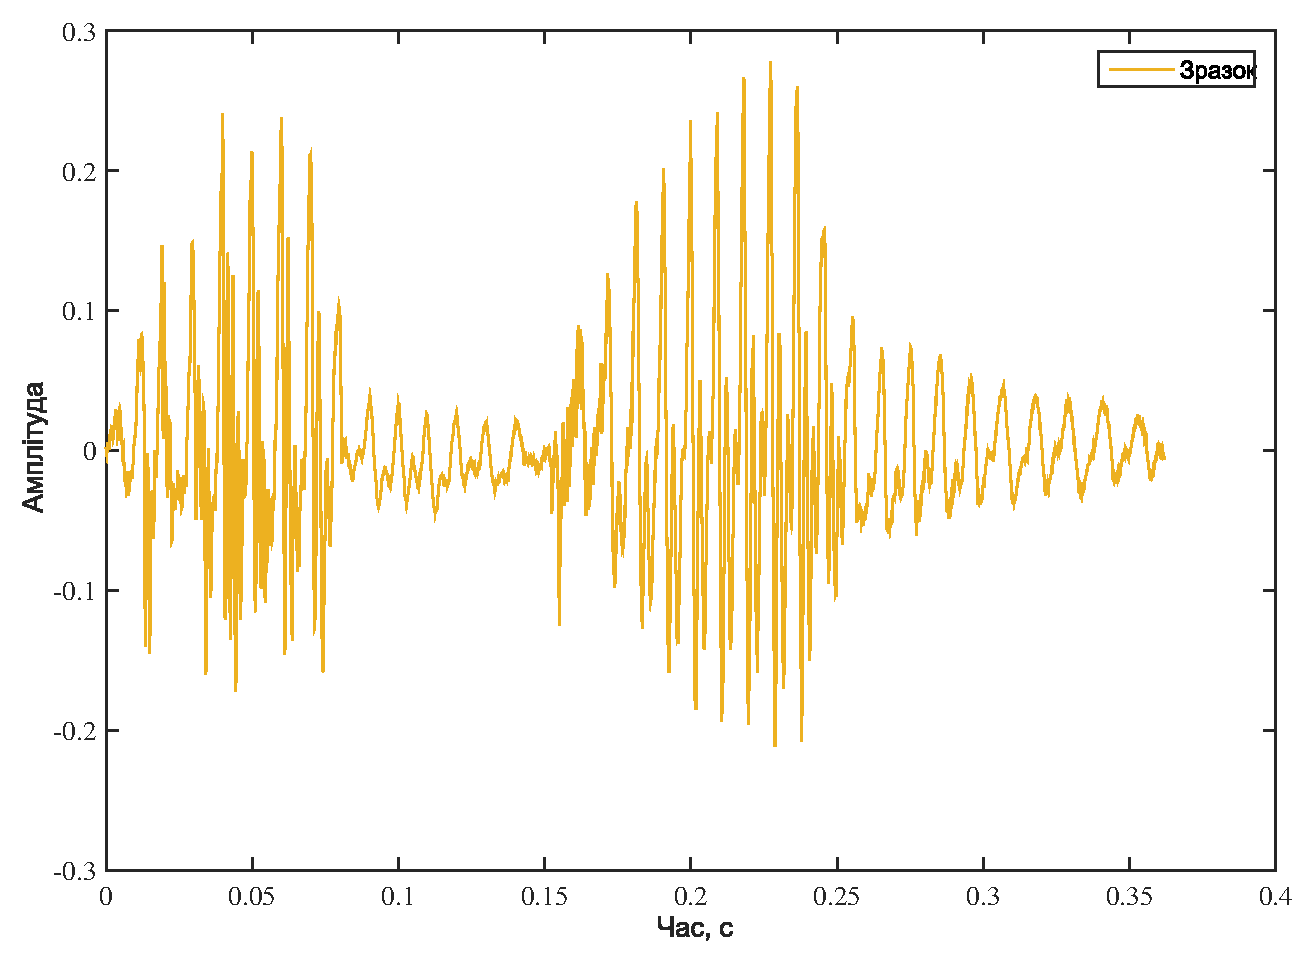
\includegraphics[width=0.8\textwidth]{audio_template.eps}
        }

        \subfloat[Коротко"=часова енергія]{%
            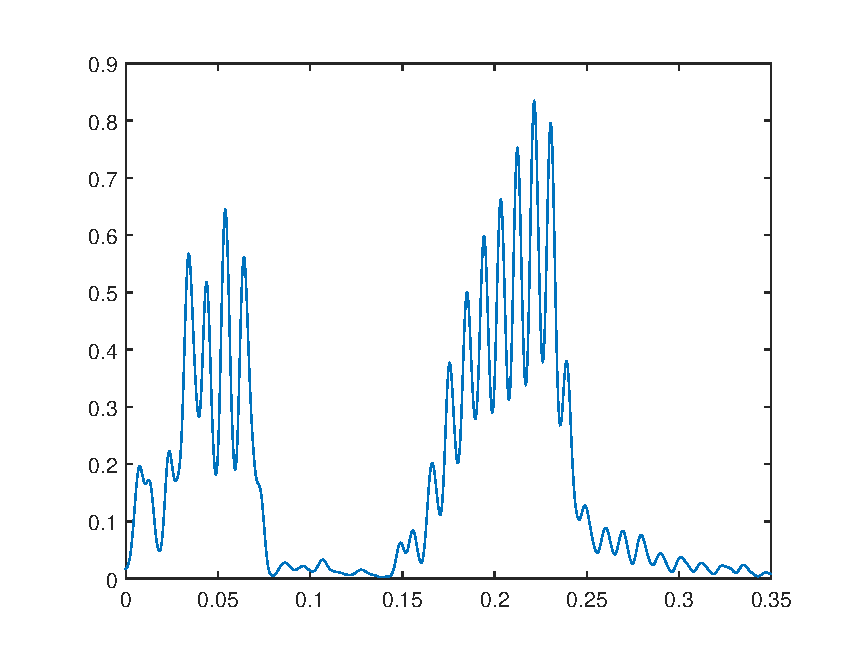
\includegraphics[width=0.8\textwidth]{audio_template_energy.eps}
        }
        \caption{Приклад обчислення коротко"=часової енергії}
        \label{fig:ste-example}
    \end{figure}

    Як було зазначено, розмір вікна зазвичай обирається 10--30 мілісекунд, оскільки на таких проміжках енергія
    мовленнєвого сигналу вважається статичною.
    Якщо обирати розмір вікна більше за 40 мілісекунд, то отримана коротко"=часова енергія буде більш гладкою.

    Гладкість та означеність екстремумів коротко"=часової енергії також залежить від вибору вікна.

    В розділі~\ref{chap:testing} будуть розглянуті впливи обраної форми ти розміру вікна на коротко"=часову енергію.

\section{Висновки}
В цьому розділі був визначений лінійній простір над породжуючою функцією, або лінійний простір Кунченко.
Було показано, як використовуючи наближення функції елементами базису цього простору можна вирішити задачу пошуку
шаблону в цифровому сигналі.
Обраний метод має більш нечітку оцінку присутності шаблону в сигналі, ніж розглянуті в попередньому розділі.
Також були розглянуті методики, завдяки яким можна прискорити роботу методу.

В розділі~\ref{chap:testing} буде проведене тестування методу пошуку шаблонів за допомогою поліномів Кунченка як на
синтетичних прикладах, так і на мовленнєвих сигналах.

% vim: spelllang=uk,en spell filetype=tex
